\section{Experiment}
\textbf{Overview}
\\ \\
In this part we will talk about the whole experiment, lay aside the quality of the result, we mainly discuss the runtime from a grand view. We pick 30 precedents from our document set, and make an experiment to test the runtime of our algorithm in different situation. We have 3 sets of 10 precedents, 2 sets of 20 precedents, and 1 set of 30 precedents.\\
The result is as follow:\\
\begin{table}[!h]
\centering
\begin{tabular}{cccc}
\hline
Experiment&Event process&KeyGraph&MFC by CLIQUES\\
\hline
10-0&0.40&7.11&8.49\\
10-1&0.48&9.85&31.37\\
10-2&0.48&9.50&15.41\\
20-0&1.02&17.79&113.02\\
20-1&0.96&18.89&122.60\\
30-0&1.24&26.48&275.15\\
10-avg&0.45&8.82&18.42\\
20-avg&0.99&18.39&117.81\\
30-avg&1.24&26.48&275.15\\
\hline
\end{tabular}
\caption{data of runtime experiment}
\end{table}
We can find that the EVENT progress and KeyGraph algorithm is work in a linnner runtime, we the input increase, the runtime linear increases. But MFC by CLIQUE algorithm is different, when the amount of precedents increases, the runtime become very long and Increase rapidly.\\
 We can see it from a figure.\\ \\
\begin{figure}[!h]
\centering
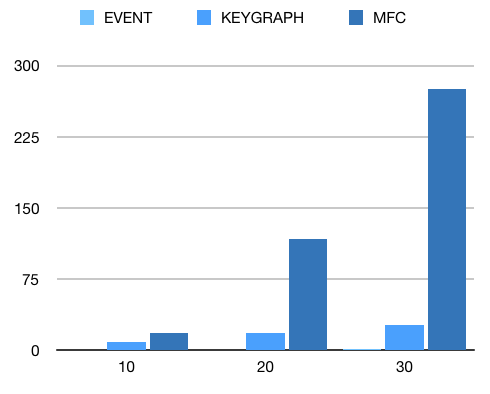
\includegraphics[width=250pt]{./pictures/0403-0.png}
\caption{statistic of runtime}
\end{figure}
After the evaluation, we mainly talk about the quality of the result in the following experiments, and what we can get from the algorithm.\\ \\
\textbf{Experiment of Short Japanese Stories}
\\ \\
We use the stories we have mentioned before, one is \begin{CJK}{UTF8}{ipxm}\textbf{あばれ鹿}\end{CJK} the other is \begin{CJK}{UTF8}{ipxm}\textbf{あやしい牛}\end{CJK}.\\
Because the stories is very short, the MFC founded is also very less, 4 result extracted:
\begin{enumerate}[*]
\item \begin{CJK}{UTF8}{ipxm}[荒らす/ヲ] [町001, 八百屋001, 田畑002]\end{CJK}
\item \begin{CJK}{UTF8}{ipxm}[持つ/ヲ] [光001, 火縄銃002]\end{CJK}
\item \begin{CJK}{UTF8}{ipxm}[困る/ガ] [若者001, 村人002]\end{CJK}
\item \begin{CJK}{UTF8}{ipxm}[現れる/ガ] [化け物001, 鹿002, 牛001, 老人001]\end{CJK}
\end{enumerate}
Although the result is not very well in this situation, we can still find some information from the result, some nouns play same role in different stories contain the information of descriptive similarity. The maximal closures will construct the descriptive pattern.
\begin{table}[!h]
\centering
\begin{tabular}{cc}
\hline
\begin{CJK}{UTF8}{ipxm}\textbf{あやしい牛}\end{CJK}&\begin{CJK}{UTF8}{ipxm}\textbf{あばれ鹿}\end{CJK}\\
\hline
\begin{CJK}{UTF8}{ipxm}町\end{CJK}&\begin{CJK}{UTF8}{ipxm}田畑\end{CJK}\\
\begin{CJK}{UTF8}{ipxm}若者\end{CJK}&\begin{CJK}{UTF8}{ipxm}村人\end{CJK}\\
\begin{CJK}{UTF8}{ipxm}光\end{CJK}&\begin{CJK}{UTF8}{ipxm}火縄銃\end{CJK}\\
\begin{CJK}{UTF8}{ipxm}牛\end{CJK}&\begin{CJK}{UTF8}{ipxm}鹿\end{CJK}\\
\hline
\end{tabular}
\caption{Similarity classes between stories}
\end{table}
\newpage
\textbf{Experiment 4-1}
\\ \\
In this experiment we use 4 similar precedents and set $\tau = 1$ to see whether there exist descriptive patterns supported by all the precedents.
\begin{table}[!h]
\centering
\begin{tabular}{cccc}
\hline
words(noun)&Event($s$)&KeyGraph($s$)&MFC($s$)\\
\hline
95423&0.22&16.77&28.89\\
\hline
\end{tabular}
\caption{4 similar Precedents}
\end{table}
51 maximal closures are extracted:
\begin{enumerate}
\item \begin{CJK}{UTF8}{ipxm}[有る/ニ, 言う/ト] [社会068, 項085, 過失092, 国保069]\end{CJK}
\item \begin{CJK}{UTF8}{ipxm}[受ける/ニ, 成る/ガ, 行う/ガ] [支部069, 株式085, 原告092, 原告068, 孤児068]\end{CJK}
\item \begin{CJK}{UTF8}{ipxm}[する/ニ, 受ける/カラ, 有る/ニ] [証券085, 国068, 原告092, 国保069]\end{CJK}
\item \begin{CJK}{UTF8}{ipxm}[する/ト, する/ヲ, つく/ニ, 成る/ガ, 認める/ガ] [義務068, 額085, 責任092, 被告069]\end{CJK}
\item \begin{CJK}{UTF8}{ipxm}[する/ト, つく/ニ, 成る/ガ, 有る/ガ, 認める/ガ] [義務068, 号085, 責任092, 被告069]\end{CJK}
\item \begin{CJK}{UTF8}{ipxm}[する/ガ, 主張/ガ, 求める/ガ, 生じる/ニ, 被る/ガ, 言う/ガ, 請求/ガ] [原告085, 原告092, 原告068, 国保069]\end{CJK}
\item \begin{CJK}{UTF8}{ipxm}[する/ガ, 有る/ニ, 認める/ニ, 請求/ガ] [原告085, 原告092, 被告069, 国068]\end{CJK}
\item \begin{CJK}{UTF8}{ipxm}[する/ガ, 主張/ガ, 有る/ニ, 求める/ガ, 生じる/ニ, 認める/ニ] [原告085, 原告092, 被告069, 被告068]\end{CJK}
\item \begin{CJK}{UTF8}{ipxm}[する/ガ, 検討/ガ, 求める/ガ, 生じる/ニ, 認める/ニ] [原告085, 原告092, 被告069, 孤児068]\end{CJK}
\item \begin{CJK}{UTF8}{ipxm}[する/ガ, する/ニ, 認める/ガ] [書069, 額085, 原告092, 過失092, 権利068, 号085, 士092]\end{CJK}
\item \begin{CJK}{UTF8}{ipxm}[する/ガ, つく/ニ, 成る/ガ] [法068, 株式085, 組合085, 額085, 責任092, 号085, 被告069]\end{CJK}
\item \begin{CJK}{UTF8}{ipxm}[する/ガ, 定める/ガ, 成る/ガ, 負う/ガ] [法068, 項085, 原告092, 国保069, 被告069]\end{CJK}
\item \begin{CJK}{UTF8}{ipxm}[する/ガ, 作成/ガ, 認識/ガ] [省068, 書085, 原告092, 国保069]\end{CJK}
\item \begin{CJK}{UTF8}{ipxm}[する/ガ, する/ニ, する/ヲ, 有る/ガ, 要求/ガ, 負う/ガ] [国068, 士092, 項085, 国保069]\end{CJK}
\item \begin{CJK}{UTF8}{ipxm}[する/ガ, する/ヲ, 有る/ガ, 要求/ガ, 認める/ニ, 負う/ガ] [国068, 士092, 項085, 被告069]\end{CJK}
\item \begin{CJK}{UTF8}{ipxm}[する/ガ, する/ニ, する/ヲ, 成る/ガ, 有る/ガ, 有る/ニ, 負う/ガ] [国068, 項085, 原告092, 国保069]\end{CJK}
\item \begin{CJK}{UTF8}{ipxm}[する/ガ, する/ヲ, 成る/ガ, 有る/ガ, 有る/ニ, 認める/ニ, 負う/ガ] [国068, 被告069, 項085, 原告092]\end{CJK}
\item \begin{CJK}{UTF8}{ipxm}[する/ガ, する/ニ, 受ける/カラ, 成る/ガ, 有る/ガ, 負う/ガ] [国068, 号085, 原告092, 国保069]\end{CJK}
\item \begin{CJK}{UTF8}{ipxm}[する/ガ, する/ニ, 含む/ガ, 有る/ニ] [国068, 書085, 原告092, 業務069]\end{CJK}
\item \begin{CJK}{UTF8}{ipxm}[する/ガ, する/ニ, 有る/ニ, 認識/ガ] [国068, 書085, 原告092, 国保069]\end{CJK}
\item \begin{CJK}{UTF8}{ipxm}[する/ガ, する/ヲ, 成る/ニ, 有る/ガ] [条092, 人068, 円085, 国保069]\end{CJK}
\item \begin{CJK}{UTF8}{ipxm}[する/ガ, する/ヲ, よる/ニ, 有る/ガ] [条092, 頁069, 項085, 者068]\end{CJK}
\item \begin{CJK}{UTF8}{ipxm}[する/ガ, 持つ/ヲ] [甲069, 株式085, 場092, 家族068, 責任092]\end{CJK}
\item \begin{CJK}{UTF8}{ipxm}[する/ガ, する/ト, 要する/ガ] [場092, 国保069, 項085, 人068]\end{CJK}
\item \begin{CJK}{UTF8}{ipxm}[する/ガ, する/ト, する/ニ, する/ヲ, 主張/ガ, 成る/ガ] [額085, 国保069, 原告092, 権利068]\end{CJK}
\item \begin{CJK}{UTF8}{ipxm}[する/ガ, する/ト, する/ヲ, 主張/ガ, 成る/ガ, 認める/ガ] [額085, 被告069, 原告092, 権利068]\end{CJK}
\item \begin{CJK}{UTF8}{ipxm}[する/ガ, する/ト, する/ヲ, 主張/ガ, 認める/ニ] [額085, 被告068, 原告092, 被告069]\end{CJK}
\item \begin{CJK}{UTF8}{ipxm}[する/ガ, する/ト, する/ヲ, つく/ニ, 認める/ガ] [額085, 条068, 責任092, 被告069]\end{CJK}
\item \begin{CJK}{UTF8}{ipxm}[する/ガ, する/ト, する/ヲ, 当たる/ガ, 成る/ガ] [線092, 被告069, 権利068, 円085, 者068]\end{CJK}
\item \begin{CJK}{UTF8}{ipxm}[する/ガ, する/ト, する/ヲ, 受ける/ガ, 成る/ガ] [株085, 原告092, 人068, 孤児068, 権利068, 者068, 国保069, 被告069]\end{CJK}
\item \begin{CJK}{UTF8}{ipxm}[する/ガ, する/ト, する/ニ, する/ヲ, 含む/ガ] [業務069, 円085, 原告092, 権利068, 者068]\end{CJK}
\item \begin{CJK}{UTF8}{ipxm}[する/ガ, する/ト, する/ヲ, 含む/ガ, 成る/ガ, 有る/ガ] [人068, 円085, 者068, 権利068, 原告092, 被告069]\end{CJK}
\item \begin{CJK}{UTF8}{ipxm}[する/ガ, する/ト, する/ニ, する/ヲ, 成る/ガ, 有る/ガ, 言う/ト] [過失092, 項085, 権利068, 国保069, 者068]\end{CJK}
\item \begin{CJK}{UTF8}{ipxm}[する/ガ, する/ト, する/ニ, する/ヲ, 成る/ガ, 有る/ガ, 生じる/ニ, 負う/ガ] [項085, 国保069, 孤児068, 原告092]\end{CJK}
\item \begin{CJK}{UTF8}{ipxm}[する/ガ, する/ト, する/ヲ, 成る/ガ, 有る/ガ, 生じる/ニ, 認める/ニ, 負う/ガ] [被告069, 項085, 原告092, 孤児068]\end{CJK}
\item \begin{CJK}{UTF8}{ipxm}[する/ガ, する/ト, する/ヲ, 定める/ガ, 有る/ガ, 有る/ニ, 生じる/ニ, 認める/ニ, 負う/ガ] [被告068, 項085, 原告092, 被告069]\end{CJK}
\item \begin{CJK}{UTF8}{ipxm}[する/ガ, する/ト, 成る/ガ, 有する/ガ, 行う/ガ] [株式085, 原告092, 被告069, 国保069, 孤児068, 者068]\end{CJK}
\item \begin{CJK}{UTF8}{ipxm}[する/ガ, する/ト, 主張/ガ, 行う/ガ] [株式085, 被告068, 原告092, 被告069, 国保069]\end{CJK}
\item \begin{CJK}{UTF8}{ipxm}[する/ガ, する/ト, 有する/ガ, 認める/ガ] [株式085, 条068, 被告069, 原告092]\end{CJK}
\item \begin{CJK}{UTF8}{ipxm}[する/ガ, する/ト, 成る/ト] [システム069, 額085, 者068, 権利068, 円085, 列車092, 人068, 孤児068]\end{CJK}
\item \begin{CJK}{UTF8}{ipxm}[する/ガ, する/ト, 有る/ガ, 認める/ガ, 負う/ガ] [号085, 士092, 原告092, 条068, 被告069]\end{CJK}
\item \begin{CJK}{UTF8}{ipxm}[する/ガ, する/ト, する/ニ, 成る/ガ, 有る/ガ, 言う/ガ] [号085, 者068, 原告092, 国保069]\end{CJK}
\item \begin{CJK}{UTF8}{ipxm}[する/ガ, する/ト, 成る/ガ, 有る/ガ, 認める/ガ] [号085, 責任092, 被告069, 原告092, 過失092, 権利068]\end{CJK}
\item \begin{CJK}{UTF8}{ipxm}[する/ガ, する/ト, 支払う/ガ, 有る/ガ, 負う/ガ] [号085, 被告068, 原告092, 国保069, 被告069]\end{CJK}
\item \begin{CJK}{UTF8}{ipxm}[する/ガ, する/ト, つく/ニ, 有る/ガ, 認める/ガ] [号085, 条068, 被告069, 責任092]\end{CJK}
\item \begin{CJK}{UTF8}{ipxm}[する/ガ, 主張/ガ, 成る/ガ, 有する/ガ, 行う/ガ] [原告068, 株式085, 原告092, 国保069, 被告069]\end{CJK}
\item \begin{CJK}{UTF8}{ipxm}[する/ガ, する/ヲ, 占める/ガ, 成る/ガ, 有る/ガ] [原告068, 被告069, 過失092, 円085]\end{CJK}
\item \begin{CJK}{UTF8}{ipxm}[する/ガ, する/ニ, 含む/ガ, 行う/ニ] [書085, 業務069, 原告092, 者068]\end{CJK}
\item \begin{CJK}{UTF8}{ipxm}[する/ガ, 含む/ガ, 有る/ニ, 行う/ニ, 認める/ニ] [書085, 被告068, 原告092, 被告069]\end{CJK}
\item \begin{CJK}{UTF8}{ipxm}[する/ガ, 提出/ガ, 行う/ニ, 認める/ニ] [書085, 士092, 被告069, 者068]\end{CJK}
\item \begin{CJK}{UTF8}{ipxm}[支払う/ガ, 求める/ニ, 負う/ガ] [被告085, 国保069, 被告068, 被告092, 被告069]\end{CJK}
\end{enumerate}
We can pick some closures to bulid part of our descriptive pattern manual, because the document is very similar, the pattern may very long, we list part of them.
\begin{figure}[!h]
\centering
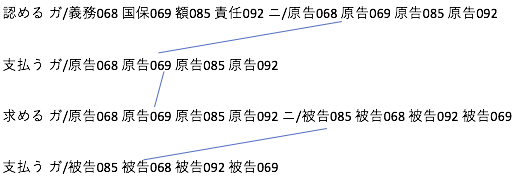
\includegraphics[width=250pt]{./pictures/0403-1.png}
\caption{Part of Descriptive patterns}
\end{figure}
\newpage
\textbf{Experiment 4-2}
\\ \\
In this experiment we use 4 precedents which seem very different from each other and set $\tau = 1/2$ to see whether our algorithm can extract descriptive patterns among multiple precedents.
\begin{table}[!h]
\centering
\begin{tabular}{cccc}
\hline
words(noun)&Event($s$)&KeyGraph($s$)&MFC($s$)\\
\hline
6974&0.03&0.40&0.09\\
\hline
\end{tabular}
\caption{4 very differnet Precedents}
\end{table}
Closures are extracted:
\begin{enumerate}
\item \begin{CJK}{UTF8}{ipxm}[受ける/ニ, 変更/ニ] [事件007, 人000]\end{CJK}
\item \begin{CJK}{UTF8}{ipxm}[喪失/ニ, 死亡/ニ] [事故077, 行為000]\end{CJK}
\item \begin{CJK}{UTF8}{ipxm}[主張/ガ, 居住/ガ, 請求/ニ] [被告007, 被告005]\end{CJK}
\item \begin{CJK}{UTF8}{ipxm}[する/ト, する/ニ] [権000, 原告007]\end{CJK}
\item \begin{CJK}{UTF8}{ipxm}[する/ト, 主張/ガ, 受ける/ガ, 受ける/ニ, 求める/ガ, 求める/ニ, 知る/ガ] [被告005, 原告007]\end{CJK}
\item \begin{CJK}{UTF8}{ipxm}[する/ト, 言う/ガ] [逸失利益000, 原告007]\end{CJK}
\item \begin{CJK}{UTF8}{ipxm}[する/ト, 考える/ガ] [逸失利益000, 口007]\end{CJK}
\item \begin{CJK}{UTF8}{ipxm}[する/ト, 成る/ガ, 生じる/ニ] [利益000, 原告007]\end{CJK}
\item \begin{CJK}{UTF8}{ipxm}[受ける/ニ, 請求/ニ] [行為007, 被告005]\end{CJK}
\item \begin{CJK}{UTF8}{ipxm}[求める/ガ, 求める/ニ, 請求/ニ] [人077, 被告005]\end{CJK}
\item \begin{CJK}{UTF8}{ipxm}[求める/ニ, 負う/ニ] [人077, 者000]\end{CJK}
\item \begin{CJK}{UTF8}{ipxm}[控訴/ガ, 求める/ガ, 求める/ニ] [人077, 原告007]\end{CJK}
\item \begin{CJK}{UTF8}{ipxm}[受ける/ガ, 受ける/ニ, 命ずる/ニ, 支払う/ガ, 求める/ガ] [人000, 原告007]\end{CJK}
\item \begin{CJK}{UTF8}{ipxm}[取得/ガ, 受ける/ガ, 受ける/ニ, 求める/ガ] [人000, 被告005]\end{CJK}
\item \begin{CJK}{UTF8}{ipxm}[有る/ガ, 生じる/ニ] [者000, 過失077]\end{CJK}
\item \begin{CJK}{UTF8}{ipxm}[受ける/ガ, 求める/ニ, 生じる/ニ, 被る/ガ, 負う/ガ] [者000, 原告007]\end{CJK}
\item \begin{CJK}{UTF8}{ipxm}[取得/ガ, 受ける/ガ, 求める/ニ] [者000, 被告005]\end{CJK}
\item \begin{CJK}{UTF8}{ipxm}[成る/ガ, 言う/ガ] [額000, 原告007]\end{CJK}
\item \begin{CJK}{UTF8}{ipxm}[する/ガ, する/ヲ, 言う/ガ] [額000, 事件005]\end{CJK}
\item \begin{CJK}{UTF8}{ipxm}[受ける/ニ, 言う/ガ] [事件005, 原告007]\end{CJK}
\end{enumerate}
Although the document are very different, we can still extract similarity classes between two of them, they can also build descriptive patterns.
\begin{figure}[!h]
\centering
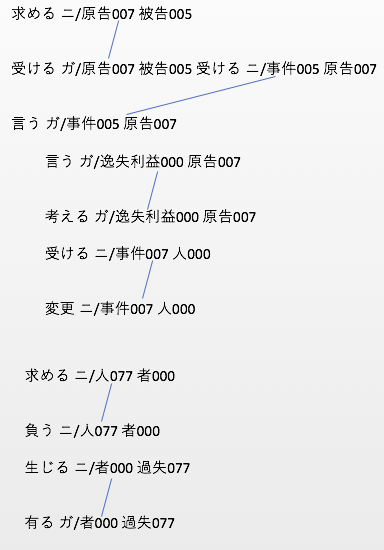
\includegraphics[width=250pt]{./pictures/0403-2.png}
\caption{Part of Descriptive patterns between different documents}
\end{figure}
\newpage
\textbf{Experiment 4-3}
\\ \\
In this experiment we use 3 precedents, two of them are similar ones and set $\tau = 2/3$. The propose is to see whether our algorithm can find similar ones between a document set.
\begin{table}[!h]
\centering
\begin{tabular}{cccc}
\hline
words(noun)&Event($s$)&KeyGraph($s$)&MFC($s$)\\
\hline
76083&0.15&10.31&8.27\\
\hline
\end{tabular}
\caption{3 Precedents include 2 similar ones}
\end{table}
Closures are extracted:
\begin{enumerate}
\item \begin{CJK}{UTF8}{ipxm}[する/デ, 取る/ニ, 有る/ニ] [駅092, 社会068]\end{CJK}
\item \begin{CJK}{UTF8}{ipxm}[する/ヲ, 取る/ニ, 書く/ニ, 有る/ガ, 設置/ニ, 連絡/ニ] [駅092, 省068]\end{CJK}
\item \begin{CJK}{UTF8}{ipxm}[する/ニ, する/ヲ, 取る/ニ, 成る/ガ, 有る/ガ, 発生/ガ, 至る/ニ, 行う/ニ] [駅092, 孤児068]\end{CJK}
\item \begin{CJK}{UTF8}{ipxm}[する/ニ, する/ヲ, 成る/ガ, 有る/ガ, 有る/ニ, 行う/デ] [駅092, 国068]\end{CJK}
\item \begin{CJK}{UTF8}{ipxm}[する/ヲ, 有る/ガ, 有る/ニ, 発生/ガ, 行う/ニ] [駅092, 被告068]\end{CJK}
\item \begin{CJK}{UTF8}{ipxm}[する/ニ, する/ヲ, 居る/ニ, 行う/ニ, 設置/ニ] [駅092, センター068]\end{CJK}
\item \begin{CJK}{UTF8}{ipxm}[する/ニ, する/ヲ, 成る/ガ, 置く/ニ, 行う/ニ] [駅092, 問題068]\end{CJK}
\item \begin{CJK}{UTF8}{ipxm}[する/デ, 受ける/ニ, 得る/ニ, 有る/ニ, 確立/ニ] [社会068, 原告092]\end{CJK}
\item \begin{CJK}{UTF8}{ipxm}[する/デ, 出来る/ニ, 取る/ニ, 持つ/ヲ] [社会068, 場092]\end{CJK}
\item \begin{CJK}{UTF8}{ipxm}[有る/ニ, 言う/ト] [社会068, 過失092]\end{CJK}
\item \begin{CJK}{UTF8}{ipxm}[持つ/ヲ, 言う/ト] [社会068, 責任092]\end{CJK}
\item \begin{CJK}{UTF8}{ipxm}[受ける/ニ, 発する/ガ] [騒音025, 原告092]\end{CJK}
\item \begin{CJK}{UTF8}{ipxm}[有る/ガ, 有る/ニ, 生じる/ニ, 発生/ガ, 発生/ニ, 行う/ニ, 認める/ニ] [事故092, 被告068]\end{CJK}
\item \begin{CJK}{UTF8}{ipxm}[する/ニ, 判断/ニ, 有る/ガ, 死亡/デ, 死亡/ニ, 生じる/ニ, 発生/ガ, 至る/ニ, 行う/ニ, 認める/ニ] [事故092, 者068]\end{CJK}
\item \begin{CJK}{UTF8}{ipxm}[する/ニ, 判断/ニ, 取る/ニ, 周知/ニ, 有る/ガ, 生じる/ニ, 発生/ガ, 発生/ヲ, 至る/ニ, 行う/ニ, 認める/ニ] [事故092, 孤児068]\end{CJK}
\item \begin{CJK}{UTF8}{ipxm}[する/ニ, 存在/ニ, 有る/ガ, 生じる/ニ, 発生/ガ, 発生/ニ] [事故092, 原告068]\end{CJK}
\item \begin{CJK}{UTF8}{ipxm}[知る/ヲ, 行う/ニ] [事故092, 身元068]\end{CJK}
\item \begin{CJK}{UTF8}{ipxm}[行う/ガ, 述べる/ガ] [谷092, 孤児068]\end{CJK}
\item \begin{CJK}{UTF8}{ipxm}[する/ニ, する/ヲ, 受ける/ニ, 行う/ガ, 行う/ニ, 設置/ガ, 運営/ガ] [センター068, 原告092]\end{CJK}
\item \begin{CJK}{UTF8}{ipxm}[行う/ガ, 行う/ニ, 設置/ガ, 設置/ニ] [センター068, 県092]\end{CJK}
\item \begin{CJK}{UTF8}{ipxm}[する/ニ, 出来る/ニ, 居る/ニ, 行う/ニ, 設置/ヲ] [センター068, 場092]\end{CJK}
\item \begin{CJK}{UTF8}{ipxm}[する/ヲ, 判断/ガ, 成る/ト, 持つ/カラ, 行う/ニ] [円092, 者068]\end{CJK}
\item \begin{CJK}{UTF8}{ipxm}[する/ヲ, 行う/ニ, 鳴る/ト] [円092, 家族068]\end{CJK}
\item \begin{CJK}{UTF8}{ipxm}[する/ヲ, 主張/ガ, 成る/ト] [円092, 権利068]\end{CJK}
\item \begin{CJK}{UTF8}{ipxm}[する/ヲ, 認める/ト] [円092, 義務068]\end{CJK}
\item \begin{CJK}{UTF8}{ipxm}[する/ト, する/ニ, する/ヲ, 取る/ガ, 成る/ガ, 指摘/ガ, 行う/ニ, 認識/ガ, 負う/ガ] [問題068, 原告092]\end{CJK}
\item \begin{CJK}{UTF8}{ipxm}[する/ト, する/ニ, する/ヲ, 取る/ガ, 提出/ガ, 行う/ニ, 認識/ガ, 負う/ガ] [問題068, 士092]\end{CJK}
\item \begin{CJK}{UTF8}{ipxm}[する/ト, する/ニ, する/ヲ, 成る/ガ, 起こす/ニ] [問題068, 過失092]\end{CJK}
\item \begin{CJK}{UTF8}{ipxm}[する/ト, 成る/ガ, 提出/ガ, 置く/ニ, 行う/ニ] [問題068, 県092]\end{CJK}
\item \begin{CJK}{UTF8}{ipxm}[する/ト, する/ニ, 置く/ニ, 行う/ニ] [問題068, 場092]\end{CJK}
\item \begin{CJK}{UTF8}{ipxm}[受ける/カラ, 受ける/ガ, 求める/カラ] [住民025, 原告092]\end{CJK}
\item \begin{CJK}{UTF8}{ipxm}[する/ト, する/ヲ, つく/ニ, 合う/ガ, 履行/ヲ, 怠る/ヲ, 有る/ガ, 規定/ガ, 認める/ヲ, 課す/ヲ, 課する/ヲ, 負う/ヲ, 違反/ニ] [義務068, 義務092]\end{CJK}
\item \begin{CJK}{UTF8}{ipxm}[する/ト, する/ヲ, 主張/ヲ, 存在/ガ, 成る/ガ, 有る/ガ, 認める/ガ, 認める/ヲ] [義務068, 過失092]\end{CJK}
\item \begin{CJK}{UTF8}{ipxm}[する/ト, する/ヲ, つく/ニ, 成る/ガ, 有る/ガ, 認める/ガ, 認める/ヲ, 負う/ヲ] [義務068, 責任092]\end{CJK}
\item \begin{CJK}{UTF8}{ipxm}[する/ト, する/ヲ, 合う/ガ, 成る/ガ, 有る/ガ, 認める/ガ, 課する/ガ] [義務068, 原告092]\end{CJK}
\item \begin{CJK}{UTF8}{ipxm}[する/ヲ, 定める/ヲ, 有る/ガ, 規定/ガ, 規定/ニ, 規定/ヲ, 違反/ニ] [義務068, 条092]\end{CJK}
\item \begin{CJK}{UTF8}{ipxm}[発生/ガ, 認める/ガ] [義務068, 本件092]\end{CJK}
\item \begin{CJK}{UTF8}{ipxm}[有る/ガ, 考慮/ヲ] [義務068, 要素025]\end{CJK}
\item \begin{CJK}{UTF8}{ipxm}[締結/ガ, 行う/デ, 認める/ニ] [本件092, 国068]\end{CJK}
\item \begin{CJK}{UTF8}{ipxm}[発生/ガ, 認める/ニ, 違反/ガ] [本件092, 被告068]\end{CJK}
\item \begin{CJK}{UTF8}{ipxm}[発生/ガ, 至る/ガ, 認める/ニ] [本件092, 孤児068]\end{CJK}
\item \begin{CJK}{UTF8}{ipxm}[共通/ガ, 有る/ガ] [要素025, 権利068, 原告068]\end{CJK}
\item \begin{CJK}{UTF8}{ipxm}[する/ガ, 定める/ガ, 定める/ニ, 規定/ガ, 規定/ニ, 規律/ガ, 適用/ガ] [法068, 条092]\end{CJK}
\item \begin{CJK}{UTF8}{ipxm}[する/ガ, 受ける/ガ, 定める/ガ, 成る/ガ, 負う/ガ, 負う/ニ, 足る/ガ] [法068, 原告092]\end{CJK}
\item \begin{CJK}{UTF8}{ipxm}[する/ガ, 主張/ヲ, 成る/ガ, 負う/ニ] [法068, 過失092]\end{CJK}
\item \begin{CJK}{UTF8}{ipxm}[する/ガ, つく/ニ, 成る/ガ, 成立/ガ, 負う/ト, 負う/ニ] [法068, 責任092]\end{CJK}
\item \begin{CJK}{UTF8}{ipxm}[する/ガ, 発生/カラ] [法068, 場092]\end{CJK}
\item \begin{CJK}{UTF8}{ipxm}[する/ガ, 主張/ヲ, 受ける/ガ, 負う/ガ] [法068, 士092]\end{CJK}
\item \begin{CJK}{UTF8}{ipxm}[する/ガ, 有る/ガ, 至る/ニ] [被害025, 者068, 孤児068]\end{CJK}
\item \begin{CJK}{UTF8}{ipxm}[する/ガ, 受ける/ヲ, 有る/ガ] [被害025, 省068]\end{CJK}
\item \begin{CJK}{UTF8}{ipxm}[する/ガ, する/ト, 出来る/ガ, 存在/ガ, 射る/ガ, 居る/ガ, 成る/ガ, 成る/ト, 行う/ニ, 言う/ト] [列車092, 人068]\end{CJK}
\item \begin{CJK}{UTF8}{ipxm}[する/ガ, する/ト, 与える/ニ, 出す/ヲ, 出来る/ガ, 存在/ガ, 居る/ガ, 成る/ガ, 成る/ト, 発生/ガ, 編成/ヲ, 行う/ニ, 言う/ト] [列車092, 者068]\end{CJK}
\item \begin{CJK}{UTF8}{ipxm}[する/ガ, する/ト, 出す/ヲ, 出来る/ガ, 存在/ガ, 居る/ガ, 差し掛かる/ガ, 待つ/ガ, 成る/ガ, 成る/ト, 発生/ガ, 行う/ニ, 遅れる/ガ] [列車092, 孤児068]\end{CJK}
\item \begin{CJK}{UTF8}{ipxm}[する/ガ, 出来る/ガ, 居る/ガ, 待つ/ガ, 待つ/ヲ, 成る/ガ, 発生/ガ, 遅れる/ガ] [列車092, 原告068]\end{CJK}
\item \begin{CJK}{UTF8}{ipxm}[する/ガ, する/ヲ, 定める/ガ, 有る/ガ, 構成/ガ, 確認/ガ, 行う/ト] [省068, 条092]\end{CJK}
\item \begin{CJK}{UTF8}{ipxm}[する/ガ, する/ヲ, 作成/ガ, 受ける/ガ, 報告/ニ, 定める/ガ, 実施/ガ, 持つ/ガ, 有る/ガ, 行う/ト, 認める/ガ, 認識/ガ, 連絡/ニ] [省068, 原告092]\end{CJK}
\item \begin{CJK}{UTF8}{ipxm}[する/ガ, する/ヲ, 受ける/ガ, 有る/ガ, 確認/ガ, 認める/ガ, 認識/ガ] [省068, 士092]\end{CJK}
\item \begin{CJK}{UTF8}{ipxm}[する/ガ, する/ヲ, 有る/ガ, 認める/ガ, 軽視/ガ] [省068, 責任092]\end{CJK}
\item \begin{CJK}{UTF8}{ipxm}[する/ガ, する/ト, する/ヲ, つく/ニ, 有る/ガ, 規定/ガ, 違反/ニ] [義務092, 条068]\end{CJK}
\item \begin{CJK}{UTF8}{ipxm}[する/ガ, する/ト, する/ヲ, 会う/ガ, 有る/ガ, 規定/ガ, 認める/ヲ] [義務092, 者068]\end{CJK}
\item \begin{CJK}{UTF8}{ipxm}[する/ガ, する/ト, する/ヲ, 有る/ガ, 発生/ヲ, 負う/ヲ] [義務092, 孤児068]\end{CJK}
\item \begin{CJK}{UTF8}{ipxm}[する/ガ, する/ト, する/ヲ, つく/ニ, 有る/ガ, 言う/ト, 認める/ガ, 負う/ト, 負う/ニ] [条068, 責任092]\end{CJK}
\item \begin{CJK}{UTF8}{ipxm}[する/ガ, する/ト, する/ヲ, 含む/ガ, 定める/ガ, 有する/ガ, 有する/ニ, 有る/ガ, 行う/ニ, 要請/ガ, 認める/ガ, 負う/ガ, 負う/ニ, 負担/ニ] [条068, 原告092]\end{CJK}
\item \begin{CJK}{UTF8}{ipxm}[する/ガ, する/ト, する/ヲ, 実現/ガ, 有る/ガ, 生じる/カラ, 行う/ニ, 認める/ガ, 負う/ガ] [条068, 士092]\end{CJK}
\item \begin{CJK}{UTF8}{ipxm}[する/ガ, する/ト, する/ヲ, 成る/ガ, 有る/ガ, 止まる/ガ, 言う/ト, 認める/ヲ, 負う/ニ] [責任092, 者068]\end{CJK}
\item \begin{CJK}{UTF8}{ipxm}[する/ガ, する/ト, する/ニ, する/ヲ, 存在/ガ, 成る/ガ, 有る/ガ, 言う/ト, 認める/ニ, 認める/ヲ, 負う/ニ] [過失092, 者068]\end{CJK}
\item \begin{CJK}{UTF8}{ipxm}[する/ガ, する/ト, する/ニ, する/ヲ, 合わせる/ヲ, 成る/ガ, 有る/ガ, 言う/ト, 認める/ガ, 認める/ヲ] [過失092, 権利068]\end{CJK}
\item \begin{CJK}{UTF8}{ipxm}[する/ガ, する/ト, する/ニ, する/ヲ, 主張/ガ, 反する/ガ, 受ける/ガ, 含む/ガ, 成る/ガ, 有る/ガ, 認める/ガ] [原告092, 権利068]\end{CJK}
\item \begin{CJK}{UTF8}{ipxm}[する/ガ, する/ト, する/ヲ, 区分/ガ, 取る/ガ, 受ける/ガ, 含む/ガ, 居る/ガ, 成る/ガ, 有る/ガ, 果たす/ガ, 行う/ガ, 行う/ニ, 言う/ガ, 鳴る/デ] [原告092, 人068]\end{CJK}
\item \begin{CJK}{UTF8}{ipxm}[する/ガ, する/ト, する/ニ, する/ヲ, 保有/ガ, 出す/カラ, 出す/ガ, 取得/ガ, 受ける/ガ, 含む/ガ, 居る/ガ, 得る/ニ, 成る/ガ, 持つ/ガ, 提出/カラ, 有する/ガ, 有する/ニ, 有る/カラ, 有る/ガ, 求める/カラ, 求める/ガ, 生じる/ニ, 知る/ガ, 立てる/ガ, 行う/ガ, 行う/ニ, 見る/ガ, 言う/ガ, 該当/ガ, 認める/ニ, 負う/ニ] [原告092, 者068]\end{CJK}
\item \begin{CJK}{UTF8}{ipxm}[する/ガ, する/ト, する/ニ, する/ヲ, 保有/ガ, 取る/ガ, 受ける/ガ, 受ける/ニ, 居る/ガ, 得る/ニ, 成る/ガ, 拒否/ガ, 持つ/ガ, 有する/ガ, 有する/ニ, 有る/ガ, 検討/ガ, 求める/ガ, 生じる/ニ, 知る/ガ, 確立/ニ, 罹る/ガ, 至る/ガ, 行う/カラ, 行う/ガ, 行う/ニ, 行使/ガ, 認める/ニ, 負う/ガ, 負担/ガ] [原告092, 孤児068]\end{CJK}
\item \begin{CJK}{UTF8}{ipxm}[する/ガ, する/ト, する/ニ, する/ヲ, 存在/ガ, 成る/ガ, 有る/ガ, 検討/ガ, 認める/ニ] [孤児068, 過失092]\end{CJK}
\item \begin{CJK}{UTF8}{ipxm}[する/ガ, する/ト, する/ヲ, 成る/ガ, 有る/ガ, 負う/ヲ] [孤児068, 責任092]\end{CJK}
\item \begin{CJK}{UTF8}{ipxm}[する/ガ, する/ト, する/ヲ, 与える/ニ, 取る/ガ, 採る/ガ, 有る/ガ, 求める/ニ, 行う/ガ, 行う/ニ, 認める/ニ, 認識/ガ, 課する/ニ, 負う/ガ] [士092, 被告068]\end{CJK}
\item \begin{CJK}{UTF8}{ipxm}[する/ガ, する/ト, する/ヲ, 乗る/ガ, 入る/ガ, 取る/ガ, 受ける/ガ, 居る/ガ, 戻る/ガ, 有る/ガ, 聞く/カラ, 聞く/ガ, 行う/ガ, 行う/ニ, 言う/ガ] [士092, 人068]\end{CJK}
\item \begin{CJK}{UTF8}{ipxm}[する/ガ, する/ト, する/ニ, する/ヲ, 取る/ガ, 受ける/ガ, 居る/ガ, 強いる/ニ, 有る/ガ, 確認/ガ, 聞く/カラ, 行う/ガ, 行う/ニ, 認める/ニ, 負う/ガ] [士092, 孤児068]\end{CJK}
\item \begin{CJK}{UTF8}{ipxm}[する/ガ, する/ト, する/ニ, する/ヲ, 与える/ニ, 出す/カラ, 受ける/ガ, 居る/ガ, 戻る/ガ, 提出/ガ, 有る/ガ, 確認/ガ, 行う/ガ, 行う/ニ, 見る/ガ, 言う/ガ, 認める/ニ] [士092, 者068]\end{CJK}
\item \begin{CJK}{UTF8}{ipxm}[する/ガ, する/ト, する/ニ, する/ヲ, 受ける/ガ, 戻る/ガ, 有る/ガ, 認める/ガ] [士092, 権利068]\end{CJK}
\item \begin{CJK}{UTF8}{ipxm}[する/ガ, する/ト, する/ヲ, 主張/ガ, 予見/ガ, 作る/ガ, 取る/ガ, 合う/ガ, 含む/ガ, 定める/ガ, 実施/ガ, 持つ/ガ, 指摘/ガ, 挙げる/ガ, 採る/ガ, 支払う/ガ, 放棄/ガ, 有る/ガ, 有る/ニ, 果たす/ガ, 求める/ガ, 派遣/ガ, 生じる/ニ, 申し入れる/ガ, 続ける/ガ, 行う/ガ, 行う/ニ, 設置/ガ, 認める/ニ, 認識/ガ, 負う/ガ, 負う/ニ, 違反/ガ] [被告068, 原告092]\end{CJK}
\item \begin{CJK}{UTF8}{ipxm}[する/ガ, する/ニ, する/ヲ, よる/ニ, 明らかだ/ガ, 明確だ/ニ, 有る/ガ, 生じる/ニ, 確認/ガ, 確認/ニ, 行う/ニ, 規定/ガ, 規定/ニ] [条092, 者068]\end{CJK}
\item \begin{CJK}{UTF8}{ipxm}[する/ガ, する/ニ, する/ヲ, 明らかだ/ガ, 有る/ガ, 有る/ニ, 規定/ニ] [条092, 国068]\end{CJK}
\item \begin{CJK}{UTF8}{ipxm}[する/ガ, する/ニ, する/ヲ, 有る/ガ, 適用/ガ] [条092, 権利068]\end{CJK}
\item \begin{CJK}{UTF8}{ipxm}[する/ガ, する/ヲ, 定める/ガ, 定める/ニ, 有る/ガ, 行う/ニ, 規定/ガ, 規定/ニ, 規定/ヲ, 言う/ニ, 違反/ニ] [条092, 条068]\end{CJK}
\item \begin{CJK}{UTF8}{ipxm}[する/ガ, する/ヲ, 成る/ニ, 有る/ガ, 行う/ニ, 規定/ガ] [条092, 人068]\end{CJK}
\item \begin{CJK}{UTF8}{ipxm}[する/ガ, する/ニ, する/ヲ, 伝える/ニ, 反する/ガ, 受ける/カラ, 受ける/ガ, 含む/ガ, 実施/ガ, 成る/ガ, 有する/ガ, 有る/ガ, 有る/ニ, 果たす/ガ, 申し立てる/ガ, 究明/ガ, 行う/ガ, 認める/ニ, 認識/ガ, 課す/ニ, 請求/ガ, 負う/ガ, 負担/ガ, 負担/ニ, 進める/ニ, 開設/ニ] [国068, 原告092]\end{CJK}
\item \begin{CJK}{UTF8}{ipxm}[する/ガ, する/ニ, する/ヲ, 受ける/ガ, 有る/ガ, 行う/ガ, 要求/ガ, 認める/ニ, 認識/ガ, 課す/ニ, 負う/ガ] [国068, 士092]\end{CJK}
\item \begin{CJK}{UTF8}{ipxm}[する/ガ, する/ニ, する/ヲ, 主張/ヲ, 占める/ガ, 合わせる/ヲ, 成る/ガ, 有る/ガ] [原告068, 過失092]\end{CJK}
\item \begin{CJK}{UTF8}{ipxm}[する/ガ, する/ニ, する/ヲ, 主張/ガ, 出す/ガ, 取る/ガ, 取得/ガ, 受ける/ガ, 受ける/ニ, 含む/ガ, 居る/ガ, 成る/ガ, 持つ/ガ, 指摘/ガ, 挙げる/ガ, 有する/ガ, 有る/ガ, 果たす/ガ, 求める/ガ, 生じる/ニ, 確立/ガ, 続ける/ガ, 行う/ガ, 行使/ガ, 被る/ガ, 見る/ガ, 言う/ガ, 請求/ガ, 足る/ガ] [原告068, 原告092]\end{CJK}
\item \begin{CJK}{UTF8}{ipxm}[する/ガ, する/ニ, する/ヲ, 主張/ヲ, 取る/ガ, 受ける/ガ, 対する/ニ, 居る/ガ, 有る/ガ, 行う/ガ, 要求/ガ, 見る/ガ, 言う/ガ] [原告068, 士092]\end{CJK}
\item \begin{CJK}{UTF8}{ipxm}[する/ガ, する/ト, する/ヲ, 与える/ニ, 出す/カラ, 当たる/ガ, 有する/ガ, 行う/ニ] [被告092, 者068]\end{CJK}
\item \begin{CJK}{UTF8}{ipxm}[する/ガ, する/ト, する/ヲ, 与える/ニ, 主張/ガ, 委託/ガ, 履行/ガ, 支払う/ガ, 放棄/ガ, 求める/ニ, 行う/ニ, 負う/ガ] [被告092, 被告068]\end{CJK}
\item \begin{CJK}{UTF8}{ipxm}[する/ガ, する/ト, する/ヲ, 主張/ガ, 当たる/ガ] [被告092, 権利068]\end{CJK}
\item \begin{CJK}{UTF8}{ipxm}[する/ガ, する/ヲ, 主張/ガ, 付く/ガ, 存在/ニ, 有する/ガ, 知る/ニ, 行使/ガ] [被告092, 原告068]\end{CJK}
\item \begin{CJK}{UTF8}{ipxm}[する/ガ, する/ヲ, 否定/ガ, 有る/ニ, 認める/ガ] [原判決025, 原告092, 過失092]\end{CJK}
\item \begin{CJK}{UTF8}{ipxm}[する/ガ, する/デ, する/ト, する/ニ, する/ヲ, 出す/カラ, 受ける/ガ, 同意/ガ, 居る/ガ, 有る/カラ, 知る/ガ, 行う/ニ, 行う/ヲ] [家族068, 原告092]\end{CJK}
\item \begin{CJK}{UTF8}{ipxm}[する/ガ, する/ト, する/ニ, する/ヲ, 出す/カラ, 受ける/ガ, 居る/ガ, 求める/ニ, 行う/ニ] [家族068, 士092]\end{CJK}
\item \begin{CJK}{UTF8}{ipxm}[する/ガ, する/ト, する/ヲ, 持つ/ヲ] [家族068, 責任092]\end{CJK}
\item \begin{CJK}{UTF8}{ipxm}[する/ガ, する/ヲ, 報告/ニ, 設置/ニ] [線092, 省068]\end{CJK}
\item \begin{CJK}{UTF8}{ipxm}[する/ガ, する/ト, する/ニ, する/ヲ, 係る/ニ, 当たる/ガ, 成る/ガ, 適用/ニ] [線092, 者068]\end{CJK}
\item \begin{CJK}{UTF8}{ipxm}[する/ガ, する/ト, する/ニ, する/ヲ, 成る/ガ, 異なる/ニ, 至る/ガ, 適用/ニ] [線092, 孤児068]\end{CJK}
\item \begin{CJK}{UTF8}{ipxm}[する/ガ, する/ニ, する/ヲ, 存在/ニ, 成る/ガ, 認識/ニ, 適用/ニ] [線092, 原告068]\end{CJK}
\item \begin{CJK}{UTF8}{ipxm}[する/ガ, 作成/ガ, 定める/ガ, 持つ/ガ, 有る/ガ, 確認/ガ, 設置/ニ] [県092, 省068]\end{CJK}
\item \begin{CJK}{UTF8}{ipxm}[する/ガ, する/ト, 作る/ガ, 定める/ガ, 持つ/ガ, 有る/ガ, 行う/ガ, 行う/ニ, 設置/ガ, 開設/ガ] [県092, 被告068]\end{CJK}
\item \begin{CJK}{UTF8}{ipxm}[する/ガ, する/ト, 入る/ガ, 成る/ガ, 有る/ガ, 行う/ガ, 行う/ニ] [県092, 人068]\end{CJK}
\item \begin{CJK}{UTF8}{ipxm}[する/ガ, する/ト, 成る/ガ, 持つ/ガ, 有る/ガ, 確認/ガ, 行う/ガ, 行う/ニ, 表明/ガ] [県092, 孤児068]\end{CJK}
\item \begin{CJK}{UTF8}{ipxm}[する/ガ, する/ト, 出す/カラ, 出す/ガ, 成る/ガ, 持つ/ガ, 提出/ガ, 有る/ガ, 確認/ガ, 行う/ガ, 行う/ニ] [県092, 者068]\end{CJK}
\item \begin{CJK}{UTF8}{ipxm}[する/ガ, 成る/ガ, 有る/ガ, 行う/ガ, 開設/ガ] [県092, 国068]\end{CJK}
\item \begin{CJK}{UTF8}{ipxm}[する/ガ, 取る/ニ, 書く/ニ] [場092, 省068]\end{CJK}
\item \begin{CJK}{UTF8}{ipxm}[する/ガ, する/デ, する/ト, する/ニ, 持つ/ヲ, 行う/ニ] [場092, 家族068]\end{CJK}
\item \begin{CJK}{UTF8}{ipxm}[する/ガ, する/ト, する/ニ, 出来る/ニ, 派遣/ニ, 行う/ニ] [場092, 者068]\end{CJK}
\item \begin{CJK}{UTF8}{ipxm}[する/ガ, する/ト, する/ニ, 取る/ニ, 派遣/ニ, 行う/ニ] [場092, 孤児068]\end{CJK}
\item \begin{CJK}{UTF8}{ipxm}[する/ガ, する/ト, 取る/ニ, 行う/ニ, 要する/ガ] [場092, 人068]\end{CJK}
\item \begin{CJK}{UTF8}{ipxm}[する/ガ, する/ニ, 行う/デ] [場092, 国068]\end{CJK}
\end{enumerate}
113 maximal closures are extraced between 3 documents, and 108 closures between the similar ones. It is over 95\%. It means using the idea of descriptive pattern by extracting maximal closures we can differentiate similar documents from a document set.\\
Here are part of the descriptive pattern build by the two similar ones.
\begin{figure}[!h]
\centering
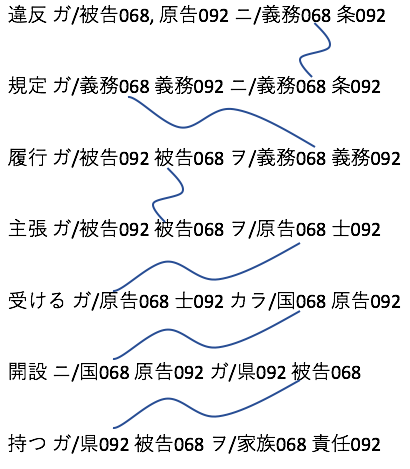
\includegraphics[width=250pt]{./pictures/0403-3.png}
\caption{Part of Descriptive patterns between similar documents}
\end{figure}
